% Preview source code

%% LyX 2.3.2 created this file.  For more info, see http://www.lyx.org/.
%% Do not edit unless you really know what you are doing.
\documentclass[oneside,english]{report}

\usepackage[T1]{fontenc}
\usepackage[utf8]{inputenc}
\usepackage{blindtext} 
\usepackage[english]{babel}
\setcounter{secnumdepth}{3}
\setcounter{tocdepth}{3}
\usepackage{amsmath}
\usepackage{amsthm}
\usepackage{float}
\usepackage{placeins}



\makeatletter
%%%%% Examples of usages %%%%%
%\todo[inline,color=green!40]{Text} % add bubble comment
%\cite{liu2019wireless} %citation of AI-Wireless from bible.bib
%%%%%%%%%%%%%%%%%%%%%%%%%%%%%% LyX specific LaTeX commands.
\providecommand{\LyX}{L\kern-.1667em\lower.25em\hbox{Y}\kern-.125emX\@}

%%%%%%%%%%%%%%%%%%%%%%%%%%%%%% Textclass specific LaTeX commands.
\numberwithin{equation}{section}
\numberwithin{figure}{section}

%%%%%%%%%%%%%%%%%%%%%%%%%%%%%% User specified LaTeX commands.
\usepackage{pgfgantt}
%%% Gantt area %%%%
\definecolor{barblue}{RGB}{153,204,254}
\definecolor{groupblue}{RGB}{51,102,254}
\definecolor{linkred}{RGB}{165,0,33} 
%%% Gantaa ared END %%%%




\usepackage[linktoc=all]{hyperref}
\usepackage{xcolor}
\usepackage{pagecolor}
\usepackage{graphicx}
\usepackage{tocbibind}
\usepackage[colorinlistoftodos]{todonotes}
\usepackage{pdfpages}

\usepackage[
backend=biber,
style=alphabetic,
sorting=ynt
]{biblatex}
\addbibresource{bibli.bib}
\usepackage{csquotes}
\usepackage{lipsum}

\usepackage[ampersand]{easylist}
\usepackage[toc,section=chapter,acronym]{glossaries}
\usepackage[toc,page]{appendix}
\makeglossaries
\newglossaryentry{iot}
{
    name=IoT,
    description={Internet of Things}
}


\newglossaryentry{sdr}
{
    name=SDR,
    description={Software Defined Radio}
}


\newglossaryentry{rssi}
{
    name=RSSI,
    description={Received Signal Strength Indication}
}


\newglossaryentry{mimo}
{
    name=MIMO,
    description={Multiple Input Multiple Output}
}


\newglossaryentry{wifi}
{
    name=WiFi,
    description={Wirless Fidelity is a family of wireless networking technologies}
}

\newglossaryentry{rcs}
{
    name=RCS,
    description={Radar Cross Section}
}

\newglossaryentry{pdp}
{
    name=PDP,
    description={Power Delay Profile}
}
\newglossaryentry{rfic}
{
    name=RFIC,
    description={Radio-frequency integrated circuit}
}
\newglossaryentry{openbts}
{
    name=OpenBTS,
    description={Open \gls{bts} is a software-based \gls{gsm}}
}
\newglossaryentry{bts}
{
    name=BTS,
    description={Base transceiver station}
}
\newglossaryentry{gsm}
{
    name=GSM,
    description={Global System for Mobile Communications known as 2nd generation of the cellular}
}
\newglossaryentry{lte}
{
    name=LTE,
    description={ Long-Term Evolution known as 4th generation of the cellular}
}
\newglossaryentry{fpga}
{
    name=FPGA,
    description={Field-programmable gate array}
}
\newglossaryentry{pcb}
{
    name=PCB,
    description={Printed circuit board}
}
\newglossaryentry{usb}
{
    name=USB,
    description={Universal Serial Bus}
}
\newglossaryentry{80211ac}
{
    name=802.11ac,
    description={IEEE 802.11ac is a wireless networking standard in the 802.11 set of protocols}
}
\newglossaryentry{gnu}
{
    name=GNU,
    description={An extensive collection of free computer software licensed with \gls{gpl}}
}
\newglossaryentry{gpl}
{
    name=GPL,
    description={The \gls{gnu} General Public License}
}
\newglossaryentry{usrp}
{
    name=USRP,
    description={Universal Software Radio Peripheral}
}
\newacronym{emag}{EM}{Electromagnetic}

\newglossaryentry{rma}
{
    name=RMA,
    description={Range Migration Algorithm}
}
\newglossaryentry{gps}
{
    name=GPS,
    description={Global Positioning System}
}
\newglossaryentry{phy}
{
    name=PHY,
    description={Physical Layer}
}
\newacronym{ap}{AP}{Access Point}

\newglossaryentry{git_git}
{
    name=Git,
    description={Distributed version control}
}

\newacronym{itu}{ITU}{International Telecommunication Union}
\newacronym{ide}{IDE}{Integrated development environment}
\newacronym{poc}{PoC}{Proof of Concept}
\newacronym{rf}{RF}{Radio Frequency}
\newacronym{ssid}{SSID}{Service Set Identifier}

\newglossaryentry{UWB}
{
    name=UWB,
    description={Ultra Wide Band}
}


\newglossaryentry{EMI}
{
    name=EMI,
    description={Electromagnetic interference}
}
\newglossaryentry{wsn}
{
    name=WSN,
    description={Wireless Sensor Network}
}
\newacronym{cw}{CW}{Continues wave}
\newacronym{dc}{DC}{Direct current}
\makeatother

\begin{document}
%-TITLE PAGE-------------------------------------------------------------------------------
%	TITLE PAGE
%----------------------------------------------------------------------------------------

\begin{titlepage}

\newcommand{\HRule}{\rule{\linewidth}{0.5mm}} % Defines a new command for the horizontal lines, change thickness here

\center % Center everything on the page
 
%----------------------------------------------------------------------------------------
%	HEADING SECTIONS
%----------------------------------------------------------------------------------------

\includegraphics[width=7cm,height=7cm,keepaspectratio]{logo-new-round1.png}\\ % Include a department/university logo - this will require the graphicx package
\textsc{\Large School of Electrical \& Computer Engineering }\\[0.5cm] % Major heading such as course name
\qquad \qquad \quad 
\includegraphics[width=3cm,height=3cm,keepaspectratio]{logo_cse1.png}\\ % Include a department/university logo - this will require the graphicx package
\iffalse
\textsc{\large Communication Systems Engineering Program}\\[0.5cm] % Minor heading such as course title
\fi
%----------------------------------------------------------------------------------------
%	TITLE SECTION
%----------------------------------------------------------------------------------------

\HRule \\[0.4cm]
{ \huge \bfseries Self-Configurable WSN using Wireless-Sensing
}\\[0.4cm] % Title of your document

 { \huge \bfseries 371-20-06}\\[0.4cm] % Title of your document
 \HRule \\[1.2cm]
%----------------------------------------------------------------------------------------
%	AUTHOR SECTION
%----------------------------------------------------------------------------------------

\begin{minipage}{0.4\textwidth}
\begin{flushleft} \large
\emph{Students:}\\
Mr. Oren \textsc{Zaharia} % Your name
\\
Mr. Efi \textsc{Dvir} % Your name
\end{flushleft}
\end{minipage}
~
\begin{minipage}{0.4\textwidth}
\begin{flushright} \large
\emph{Supervisor:} \\
Prof. Omer \textsc{Gurewitz} % Supervisor's Name
\end{flushright}
\end{minipage}\\[1cm]

% If you don't want a supervisor, uncomment the two lines below and remove the section above
%\Large \emph{Author:}\\
%John \textsc{Smith}\\[3cm] % Your name

%----------------------------------------------------------------------------------------
%	DATE SECTION
%----------------------------------------------------------------------------------------

{\large 24/01/2020}\\[0.5cm] % Date, change the \today to a set date if you want to be precise

%----------------------------------------------------------------------------------------
%	LOGO SECTION
%----------------------------------------------------------------------------------------


\includegraphics[width=3cm,height=3cm,keepaspectratio]{logo.png}\\[1cm] % Include a department/university logo - this will require the graphicx package
 
%----------------------------------------------------------------------------------------

\vfill % Fill the rest of the page with whitespace

\end{titlepage}

\iffalse
\pagestyle{empty} % No page numbers
\begin{titlepage}
Title
\definecolor{bgp}{RGB}{240,139,34}
\pagecolor{bgp} 
\end{titlepage}
\pagecolor{white} 
\fi

\chapter*{Preface}

\addcontentsline{toc}{chapter}{Preface}

\section*{About us}

\addcontentsline{toc}{section}{About us}

 Mr. Oren Zaharia (28), a senior student of the Communication
Systems Engineering program in the Ben-Gurion University of The Negev, Israel. Graduated practical engineers in electrical and computer engineering with a communication systems major. A 4 year 8200 alumni, experienced with \acrshort{rf} communication systems, signal engineering and embedded programming.
Among his hobbies are: 
Programming, bicycling, hiking, soccer, Beitar Jerusalem, history and more.
\newline
\newline
 Mr. Efi Dvir (30), a senior student of the Communication
Systems Engineering program in the Ben-Gurion University of The Negev, Israel. Graduated practical engineers in electrical and computer engineering with a communication systems major. A 4.5 year 8200 alumni, experienced with \acrshort{rf} communication systems, signal engineering and embedded programming.
Among his hobbies are: \gls{iot} sensors projects, painting, cooking, music, general craftsmanship and more.
\newline
\newline
During their B.Sc studies Mr. Efi Dvir and Mr. Oren Zaharia attended courses such as Signals and Systems, DSP, Wireless Networks Communication and more.
\newline
\newline
Together, Mr. Efi Dvir and Mr. Oren Zaharia are brewing beer in their free time as well as sometimes enjoying a nice cold brew at the local pub.

\section*{About this report}

\addcontentsline{toc}{section}{About this report}

This report describes Mr. Efi Dvir's and Mr. Oren Zaharia's progress in their Communications
Systems Engineering program's final engineering project. Throughout this document the reader might find references to articles and books who were used as an inspiration and technical basis to our project and are not Mr. Dvir and Mr. Zaharia's implementations. This report has been made using \LaTeX.

\section*{Intended audience}

\addcontentsline{toc}{section}{Intended audience}

The report is written for the academic community that want to review
and criticize our work or to be inspired or implement and learn our work.
The project in a range of final projects implementations from simple
ideas implementations to complex ideas implementations. The report
assumed that the reader have some experience and knowledge in physics,
wireless sensors networks, radio frequency, electrical wave propagation
and wireless communications. The report does not assume experience of radar techniques, our tools or any concrete knowledge in our implementation.

\section*{About this project}
This project is Mr. Efi Dvir's and Mr. Oren Zaharia's final engineering project as a partial requirements of the B.Sc  of Communications
Systems Engineering degree. This project suggests a method to infer knowledge of a sensor's surrounding environment using \gls{wifi} based wireless signals and their propagation properties. By using several methods to obtain information form \gls{wifi} signals this project strives to be able to classify the sensor's location and purpose (Temperature, pressure, humidity sensor which is located in a greenhouse in the backyard) , in order to being able to use this information to configure the sensor as a part of a whole sensor information network. The project includes both theoretical algorithmic view as well as practical hardware implementation using \gls{sdr}s. 
\addcontentsline{toc}{section}{About this project}




\renewcommand\contentsname{Table of Contents} 

\tableofcontents
\setcounter{tocdepth}{1} % fixing the problem of empty list of figures or tables

\listoffigures

\listoftables



\printglossaries



\chapter{Introduction}

\section{Background}

Smart environment is a relatively new concept, emerging in the early 1990s, where urban residents are interacting on a constant basis with informative objects, devices, sensors and actuators to seamlessly better their lives. These collect information and process it in order to provide intelligent insights to the end user and assist him in his daily routine. We treat a smart environment as an intelligent agent that perceives the state of the resident and the physical surroundings using sensors and acts on the environment using controllers in such a way that the specified performance measure is optimized \cite{Cook:2004:SET:1036248}.
Today, the number of sensors that monitor our environment is in persistent incline. With the entry of the Internet of Things (\gls{iot}) to the common household and workplaces it is becoming more and more demanding for the user administrator to manage the rising number of sensors and actuators under his responsibility. The total installed base of \gls{iot} connected devices is projected to amount to 75.44 billion worldwide by 2025, a fivefold increase in ten years. The \gls{iot}, enabled by the already ubiquitous Internet technology, is the next major step in delivering Internet’s promise of making the world a connected place \cite{iot_statista}.

\section{Motivation}

With each new sensor added to the sensor network there is a need to configure its preferences and functions in order to comply to the network’s rules and order. Whereas a new sensor placed in its place usually needs to be manually configured with the information of its location and purpose. For example, when placing a smoke sensor in the kitchen, the sensor needs to be manually configured as the kitchen sensor in the user’s system monitoring the smoke levels above the stove. If this sensor has several abilities (beside smoke detection), each with its own data feed to the information system, it may be bothersome and tedious to deploy many of these data gathering components of the network without some sort of automation. While exists some algorithms to organize the structure of the network’s traffic flow, there is a clear lack of methods to relief the end user of the task of configuring each sensor in its network manually.  
With our knowledge and passion for wireless communication, the thought of trying to engage the wireless capabilities, commonly found in many sensors, in order to assist in the configuration tasks of the user came to mind. By giving the sensor the ability to recognize and analyze its surroundings, a large amount of information could be gathered, organized and used in order to help reach an assumption on what configuration profile may be best suited for a sensor. Thus, helping the user, or even relieving him entirely of the task of sensor configuration.

\section{Goals}
\paragraph{The Primary goal} of our project is to gather new side information about the structure and composition of the device’s environment using the propagation and reflection properties of wireless signals already in use in basic wireless devices. This information would be useful to assist in the classification of the room, the operations intended for the sensor and general informative data that would better with the task of configuring the device’s function as part of the whole information network.
\paragraph{The Secondary goal} of our project is to use the gathered information to deduct insights regarding the composition of the device’s environment. By using machine learning tools and algorithms we would be able to classify the data that in turn will lead to the selection of suitable configuration profile to set to the device itself. Thus, the gathered information will be used to configure the device in the user interface.
\section{Techniques}
\subsection*{}
There are several techniques in our disposal to obtain our primary goal:
\paragraph{Radio Frequency Imaging}
Using the transmission of wireless signals via \gls{mimo} antenna array in order to compose a 2D or 3D picture of the surroundings form the reflecting signals. By applying image recognition algorithms on the generated image, we would obtain environmental data to feed to the classifier.
\paragraph{Radar}
A detection system that uses radio waves to determine the range, angle, or velocity of objects. The range and angle of the device in relation to discovered objects in the vicinity would generate data. Each object discovered would carry a \gls{rcs} that will be used as environmental data and feed to the classifier.
\paragraph{Indoor Localization}
Using data from the communications protocols used by the device (\gls{rssi} for example in figure \ref{fig:rssi_triag_ex}), we would perform location triangulation survey in relation to known sources (\gls{wifi} routers for example). This location estimation would be feed to the classifier to classify in which room the device is located. We have already examine this option in our work-space at room 512/37 as seen in figure \ref{fig:rssi_triag_512}, where is exactly described in figure \ref{fig:rssi_triag_ex}, where each letter describes the anchor name.
\begin{figure}[H]
    \centering
    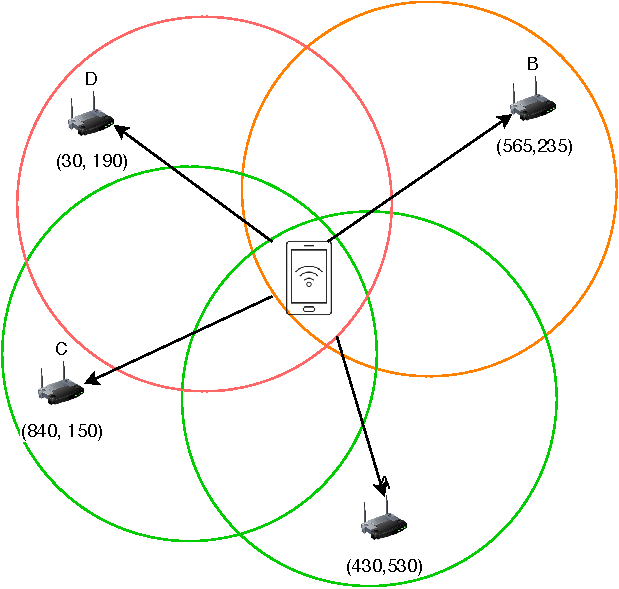
\includegraphics[width=5cm,height=5cm,keepaspectratio]{figures/rssi_triag.pdf}
    \caption{\gls{rssi} triangulation example}
    \label{fig:rssi_triag_ex}
\end{figure}
\paragraph{Radiation Holography}
Wireless data transmission systems such as \gls{wifi} or Bluetooth emit coherent light – electromagnetic waves with precisely known amplitude and phase. Propagating in space, this radiation forms  a hologram – a  two-dimensional wave-front encoding a  three-dimensional view  of all objects  traversed by the light beam \cite{Holl_2017}. Holographic data would be feed to the classifier to classify what are the objects in the room along to the room structure and size. Figure \ref{fig:holo_ex}  describes a holographic imaging process that generates 3D images using the microwave radiation of a \gls{wifi} transmitter experimented in  \cite{holography} "Holography of \gls{wifi} radiation". A space with a transmitter on the left and the resulting holographic images on the right.
\begin{figure}[H]
    \centering
    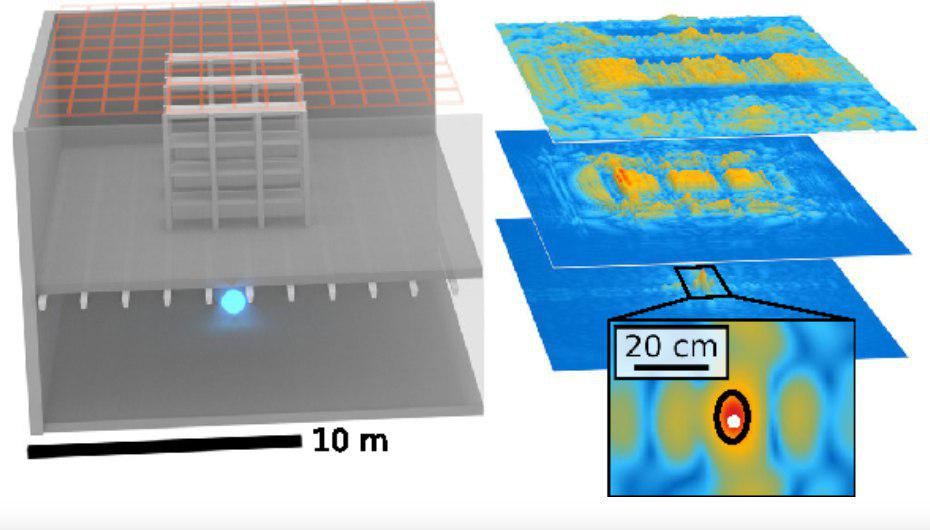
\includegraphics[width=5cm,height=5cm,keepaspectratio]{figures/fig_holg_ex.jpg}
    \caption{Holograph example}
    \label{fig:holo_ex}
\end{figure}
\paragraph{Power Delay Profile Decomposition}
The \gls{pdp} gives the intensity of a signal received through a multipath channel as a function of time delay. Each \gls{pdp} is unique and represents the channel time response.  By decomposing individual signal paths and using statistical analysis we would be able to generate data to feed to a learning machine. The figure \ref{fig:pdp_ex} gives an example to a power delay profile, where the axis time may be in nano-seconds or coarser, the power is in dB.
\begin{figure}[H]
    \centering
    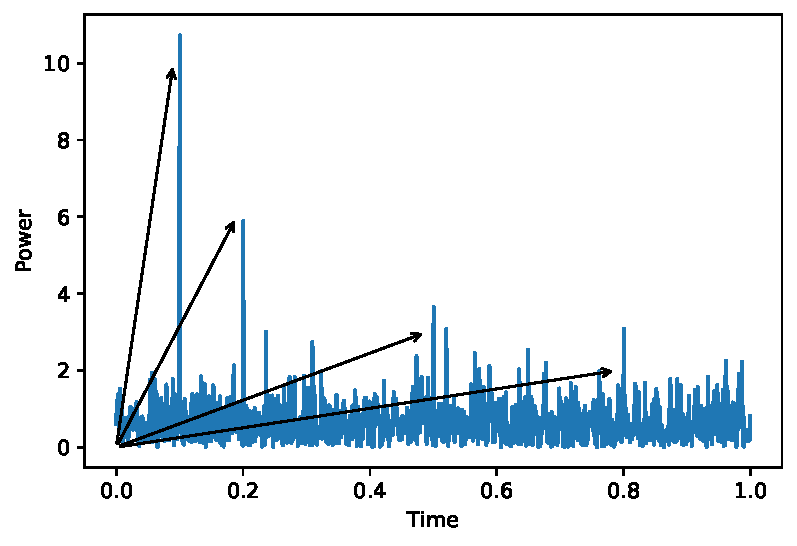
\includegraphics[height=7cm,height=5cm,keepaspectratio]{figures/pdp.pdf}
    \caption{\gls{pdp} example}
    \label{fig:pdp_ex}
\end{figure}
\subsection*{}


There are several techniques in our disposal to obtain our secondary goal:
\paragraph{Auto Encoders}an auto-encoder is a type of artificial neural network used to learn efficient data coding in an unsupervised manner \cite{wiki:xxx} By inputting general sampled signal data, we would obtain an output of data coding that in turn can be inputted into a classifier.
\paragraph{Machine learning}By using algorithms and statistical models that computer systems use to perform a specific task without using explicit instructions and by relying on patterns and inference instead, we would be able to infer properties that can assist in classifying the rooms and corresponding sensor configurations to suit it.
\paragraph{Neural networks}  - artificial neural networks may be used for predictive modeling, adaptive control and applications where they can be trained via a data-set. Self-learning resulting from experience can occur within networks, which can derive conclusions from a complex and seemingly unrelated set of information \cite{wiki:xxy}. By feeding the captured signals and information as a data-set to a pre-trained neural network we would derive conclusions regarding the device’s environment.
\chapter{The Project}
\section{Theory}

\subsection{Concepts}

In wireless radio communication, emitted signals experience a physical phenomenon known as multi-path propagation. A transmitted signal reaches the receiver after traveling by two or more paths. Walls and objects can reflect and scatter arriving signals as they cause changes in angle and time along the paths of the signal.
\paragraph{Mathematical Model \cite{wiki:multipath}}

The mathematical model of the multi-path can be presented using the
method of the impulse response used for studying linear systems.

Suppose you want to transmit a signal, ideal Dirac pulse of electromagnetic
power at time 0, i.e.

\begin{equation}
x\left(t\right)=\delta\left(t\right)    
\end{equation}

At the receiver, due to the presence of the multiple electromagnetic
paths, more than one pulse will be received, and each one of them
will arrive at different times. In fact, since the electromagnetic
signals travel at the speed of light, and since every path has a geometrical
length possibly different from that of the other ones, there are different
air travelling times (consider that, in free space, the light takes
$3\mu s$ to cross a $1km$ span). Thus, the received signal
will be expressed by (and seen in \ref{fig:multipath_ex})
\begin{equation}
y\left(t\right)=h\left(t\right)=\sum_{n-1}^{N-1}\rho_{n}e^{j\phi_{n}}\delta\left(t-\tau_{n}\right)
\end{equation}
where $N$ is the number of received impulses (equivalent to the number
of electromagnetic paths, and possibly very large), $\tau_{n}$ is
the time delay of the generic $n^{th}$ impulse, and $\rho_{n}e^{j\phi_{n}}$
represent the complex amplitude (i.e., magnitude and phase) of the
generic received pulse. Each pulse with its shift in time may be seen in figure \ref{fig:multipath_ex}. As a consequence, ${\displaystyle y\left(t\right)}$
also represents the impulse response function $h\left(t\right)$ of
the equivalent multi-path model.


\begin{figure}[h]
\centering
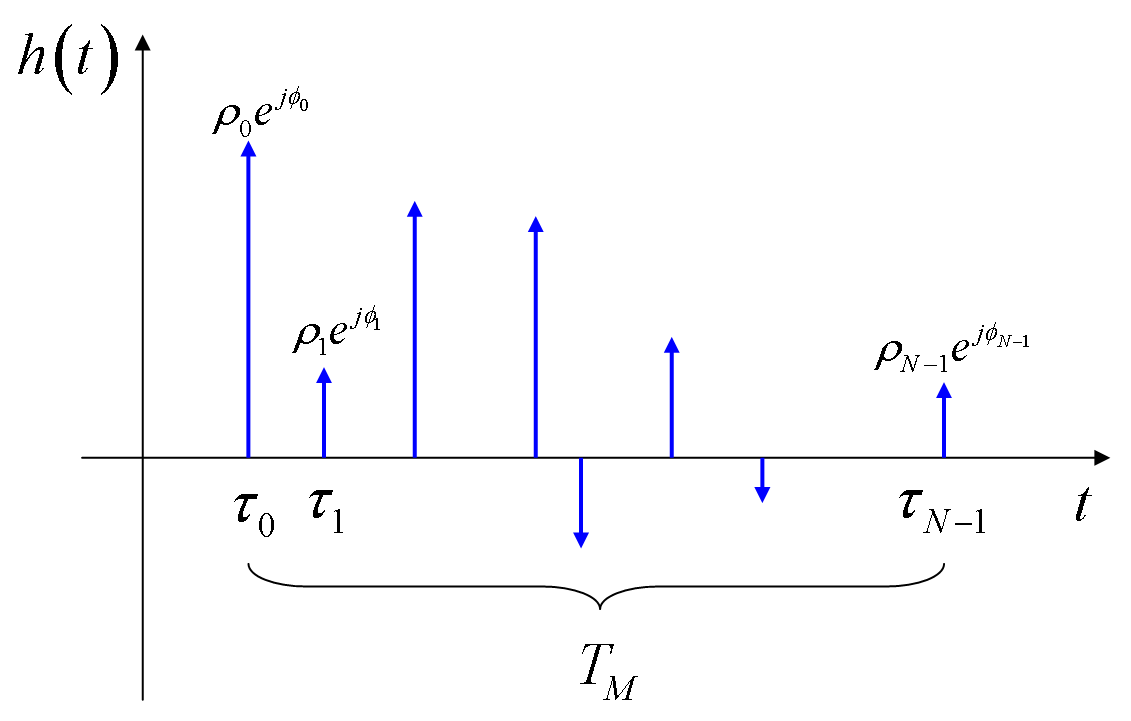
\includegraphics[width=7cm,height=7cm,keepaspectratio]{figures/Multipath_impulse_response.png}
\caption{Multi-path impulse response}
\label{fig:multipath_ex}
\end{figure}
The multi-path phenomena is always present in wireless communication, especially in indoor environments. It has been a long time that we consider multi-paths as interferences, noise, or simply nuisance. Profiles of multi-paths changes from location to location, thus, multi-path channel profile works as a unique and location-specific signature. Thus, instead of being considered as a nuisance, one can design various types of analytics based on the uniqueness of the multi-path channel state information. By fully exploiting the rich multi-path information, technology can decipher the propagation environment, revealing information that is usually disregarded. Such technology approach can enable many cutting-edge \gls{iot} applications.
\paragraph{}
The multi-path phenomena can be further exploited by using multiple-input
and multiple-output (\gls{mimo}) in the transmitting as well as in the receiving
device.

In \gls{mimo} systems, a transmitter sends multiple streams by multiple
transmit antennas. The transmit streams go through a matrix channel
which consists of all $N_{r}$ paths between the $N_{t}$ transmit
antennas at the transmitter and $N_{r}$ receive antennas at the receiver.
Then, the receiver gets the received signal vectors by the multiple
receive antennas and decodes the received signal vectors into the
original information. A narrow-band flat fading \gls{mimo} system is modelled
as
\begin{equation}
y=Hx+n    
\end{equation}


where $y$ and $x$ are the receive and transmit vectors, respectively,
and $H$ and $n$ are the channel matrix and the noise vector, respectively \cite{wiki:mimo}.
\begin{figure}[H]
\centering
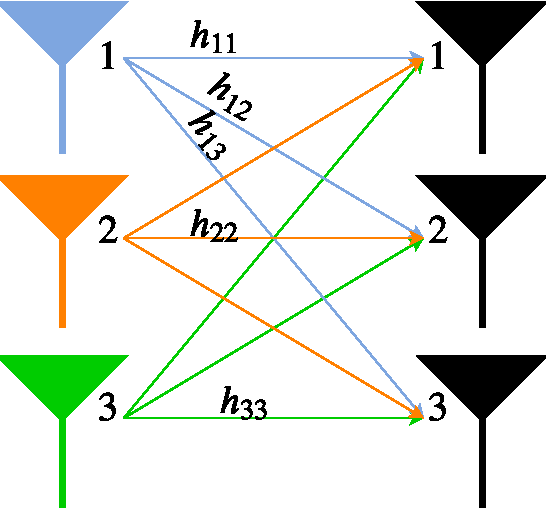
\includegraphics[width=7cm,height=7cm,keepaspectratio]{figures/MIMO_channel.pdf}
\caption{\gls{mimo} channel model}
\label{fig:mimo_channel_model}
\end{figure}
Each transmitting antenna (colored in blue orange and green in figure \ref{fig:mimo_channel_model}) is received differently in each receiving antenna (in the right side figure \ref{fig:mimo_channel_model}), thus, multiplying the amount of captured multi-path impulse responses. This expansion can further achieve unique spatial properties such as depth direction and other 3D information.

\subsection{Techniques Survey}

\paragraph{Radio Frequency Imaging}

is not a new technology, yet it has has seen little commercial success
due to the cost and power consumption of the large number of antennas and radio transceivers
required to build such a system. Huang, Nandakumar and Gollakota \cite{Huang:2014:FLW:2668332.2668344} describe the feasibility and limits of \gls{wifi} imaging by leveraging multi-path propagation. Their work introduce design and implementation which was able to identify objects inside a room (like a couch). Scott's thesis \cite{Scott:EECS-2017-191} introduces 3D microwave imaging for indoor environments which involves the use of antenna arrays, operating at microwave and millimeter-wave frequencies, for capturing images of real-world objects. His work focuses on using planar antenna arrays, operating between 17 and 26 GHz, to capture three-dimensional images of people and other objects inside a room. Scott suggests 3D microwave imaging algorithms for both dense and sparse antenna arrays as well as other algorithms such as colocated range migration algorithm \gls{rma} and a \gls{mimo} range migration algorithm which assist in the the evaluation of the 3D space. Scott also suggests a design of antennas for microwave imaging and uses the Vivaldi tapered slot antenna in his implementations. 

\begin{figure}[h]
\centering
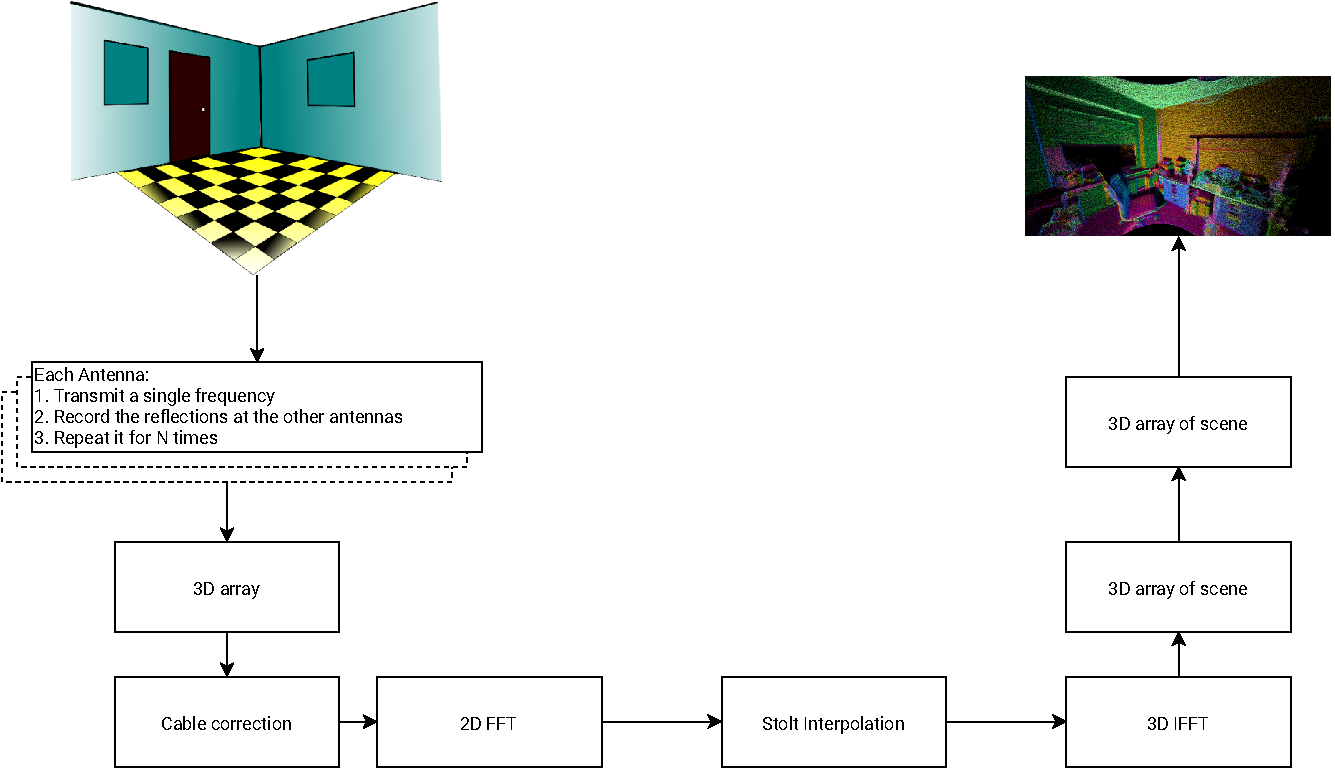
\includegraphics[width=12cm,height=7cm,keepaspectratio]{figures/RMA.pdf}
\caption{Block diagram for the colocated \gls{rma}}
\label{fig:rma_alg_ex}
\end{figure}

We intend to apply variations on Scott's work in order to comply with our hardware limitation and aspiration to use only popular protocols such as 2.4GHz  \gls{wifi} which is much lower and narrower than Scott's implementation. Yet, we need to obtain lower resolution than Scott in order to apply room analysis processing on the data acquired. By trying to combine Huang, Nandakumar and Gollakota's work with Scott's we would be able to achieve the collection of the information that we strive to obtain in order to be able to apply the inference of the surrounding environment. The algorithms that described in figure \ref{fig:rma_alg_ex}, where each block is a part in the process from raw data that had been received in its $N$ antennas to 3D array of scene.

\paragraph{Indoor Localization} is a network of devices used to locate people or objects where \gls{gps} and other satellite technologies lack precision or fail entirely.Sen, Radunovic, Choudhury and Minka \cite{sen2012spot} explore the viability of precise indoor localization using physical layer information in \gls{wifi} systems.The algorithm they suggest demonstrate localization accuracies in the granularity of 1m x 1m boxes, called spots. They show through experiments that \gls{phy} layer channel information from existing \gls{wifi} deployments can be
an indicator of location. By synthesising phase and time Lags and modeling the channel response they are able to apply clustering and classification algorithms which results in spot localization. 

\begin{figure}[h]
\centering
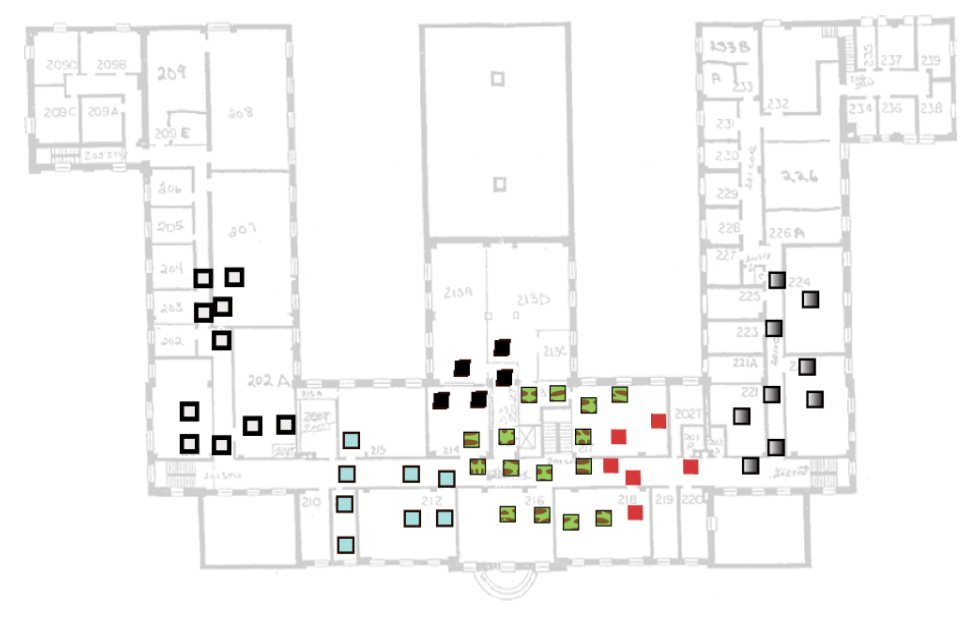
\includegraphics[width=8cm,height=7cm,keepaspectratio]{figures/spotloc.PNG}
\caption{Engineering building floor plan. Different sets of spots shown in different colors}
\label{fig:eng_bldg_floor_plan}
\end{figure}

Huang, Zheng, Xiao and Peng \cite{rssi} suggest localization based on the \gls{rssi} ranging Scope. In a \gls{rssi} based ranging algorithm, a node applies \gls{rssi} measurements to estimate its distances from the beacons, by using
a known signal propagation model. Such location information is only relative to the location of all connected \acrshort{ap}s in range. Thus, for exact localization there is a need to know where the \gls{ap}s are located.
By combining \gls{rssi} localization and the \gls{phy} localization with other data obtained from other techniques we would be able to better analyze and infer information about the device's environment.
Figure \ref{fig:eng_bldg_floor_plan} shows different sets of spots located by indoor localization using \acrshort{ap}s positions.
\begin{figure}[H]
\centering
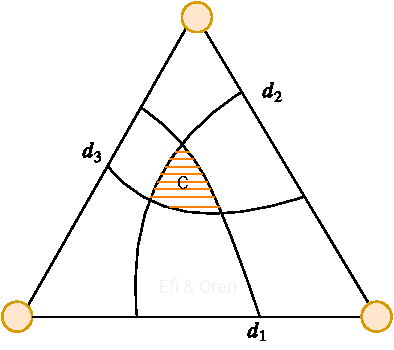
\includegraphics[width=6cm,height=6cm,keepaspectratio]{figures/rssi_regions.pdf}
\caption{Region division based on the \gls{rssi} value}
\label{fig:rssi_regions}
\end{figure}

\paragraph{Holography} is the science and practice of making holograms. Typically, a hologram is a photographic recording of a light field, rather than an image formed by a device without lens. \cite{wiki:holography}. In its pure form, holography requires the use of laser light for illuminating the subject and for viewing the finished hologram. Yet, Holl and Reinhard \cite{holography} demonstrate	a scheme	to	record	a	hologram	in	a	phase-coherent	fashion	 and	 recover	 three-dimensional	 views	 of	 objects	 and	 emitters	 and	 feeding	 the	 resulting	data	into	digital	reconstruction	algorithms.
Figure \ref{fig:holo_proc_ex}  describes a holographic imaging process that generates 3D images using the microwave radiation of a \gls{wifi} transmitter experimented in  \cite{holography} "Holography of \gls{wifi} radiation".
\begin{figure}[H]
\centering
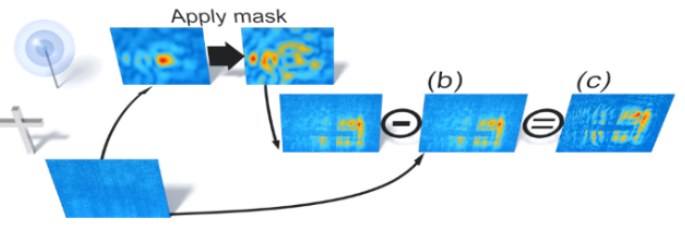
\includegraphics[width=10cm,height=6cm,keepaspectratio]{figures/holo.PNG}
\caption{Reconstruction	of objects using holography}
\label{fig:holo_proc_ex}
\end{figure}


\paragraph{Wireless Sensing} Embedded in wireless signals is information on an indoor environment which is captured during radio propagation, motivating the development of emerging wireless sensing technologies. Intelligent systems have become popular recently, in that with the help of learning they are capable of comprehending an object or even the world in the way humans do. For example, researchers have spent decades on computer vision or machine vision
systems that achieve a high-level understanding over digital images and videos that is comparable or even better than the human visual system. Can \gls{wifi} perceive an indoor environment? According to Liu and Wang\cite{liu2019wireless} the answer is yes. Applying statistical analysis on a data-set of captured signals is used for centimeter-accuracy indoor positioning and tracking, bio-metrics and vital signs estimation, motion and speed detection and more. We intend to apply similar methods on data-set of captured signals in order to create a sense of the device's environment. Many methods exist to apply indoor furniture and room recognition, Varvadoukas, Giannakidou, Gomez and Mavridis \cite{Room_Recognition} use internet-derived models and object context to achieve this. While there are plenty other methods to map and reconstruct the environment like 3D point clouds \cite{point_cloud} or set of 2D slices or just range measurements, they all relay on a data set the we would obtain from the wireless sensor.

\newpage
\section{Block Diagram}
The following block diagram describes the inner goings of a sensor device in the stages taken to infer its surrounding environment using wireless-sensing.



\begin{figure}[H]
\centering
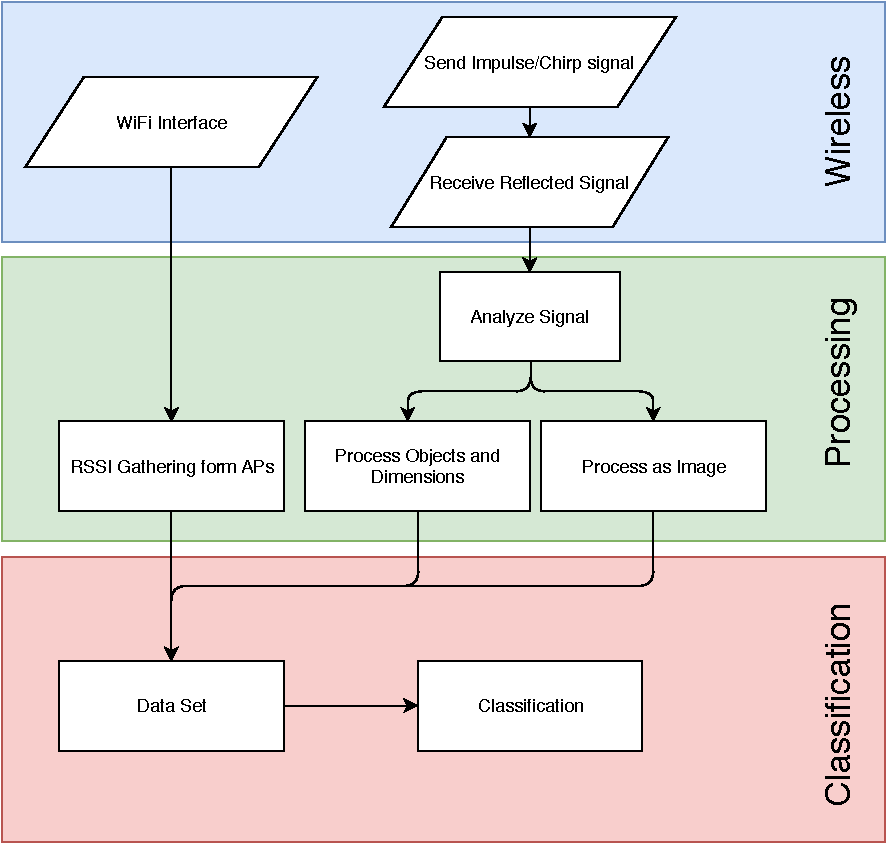
\includegraphics[width=12.5cm,height=20cm,keepaspectratio]{figures/block_diagram.pdf}
\caption{Block Diagram}
\label{fig:block_diagram_1}
\end{figure}




The Block Diagram (figure \ref{fig:block_diagram_1}) is divided in to three sections:
\begin{itemize}
    \item \textbf{Wireless Section} - The transmission and and reception of Ad-Hoc and standardized \gls{wifi} protocol signals.
    \item \textbf{Processing Section} - analyzing the received signals and processing them to an image or objects and dimensions. Creating data set from \gls{wifi} interface.
    \item \textbf{Classification} - Classifying space according to the combined created data sets.
    
\end{itemize}

\section{Practice}
\subsection{Hardware}
\paragraph{Software-Defined-Radio}
In our project we are using \gls{sdr} as our main hardware.
Software-defined radio (\gls{sdr}) is a radio communication system where components that have been traditionally implemented in hardware (e.g. mixers, filters, amplifiers, modulators/demodulators, detectors, etc.) are instead implemented by means of software on a personal computer or embedded system \cite{wiki:sdr}\cite[xxxiii]{book:139279}. While the concept of \gls{sdr} is not new, the rapidly evolving capabilities of digital electronics render practical many processes which were once only theoretically possible.
\paragraph{LimeSDR} is a low cost, open source, apps-enabled (more on that later) software defined radio (\gls{sdr}) platform that can be used to support just about any type of wireless communication standard.\cite{www:limesdr_brd}
\paragraph{Ettus \gls{usrp} B210} provides a fully integrated, single-board, Universal Software Radio Peripheral (\gls{usrp}™) platform with continuous frequency coverage from 70 MHz – 6 GHz. Designed for low-cost experimentation, it combines the AD9361 \gls{rfic} direct-conversion transceiver providing up to 56MHz of real-time bandwidth, an open and reprogrammable Spartan6 \gls{fpga}, and fast SuperSpeed USB 3.0 connectivity with convenient bus-power. Full support for the \gls{usrp} Hardware Driver™ (UHD) software allows you to immediately begin developing with \gls{gnu} Radio, prototype your own \gls{gsm} base station with \gls{openbts}, and seamless transition code from the \gls{usrp} B210 to higher performance, industry-ready \gls{usrp} platforms. An enclosure accessory kit is available to users of green \gls{pcb} devices (revision 6 or later) to assemble a protective steel case.\cite{www:ettus_b210}
\paragraph{Raspberry Pi} a series of small single-board computers. The last release of Raspberry Pi was in June 2019 with a 1.5GHz 64-bit quad core \href{https://en.wikipedia.org/wiki/ARM_Cortex-A72}{ARM Cortex-A72} processor. The board includes two \gls{usb} 3.0 ports and support \gls{80211ac} \gls{wifi}.
\subsection{Programs}
\paragraph{\gls{gnu} Radio}\gls{gnu} Radio is a free \& open-source software development toolkit that provides signal processing blocks to implement software radios. It can be used with readily-available low-cost external \acrshort{rf} hardware to create software-defined radios, or without hardware in a simulation-like environment. It is widely used in research, industry, academia, government, and hobbyist environments to support both wireless communications research and real-world radio systems \cite{www:gnuradio_about}.
The toolkit that is provided under \gls{gnu} Radio is written with C/C++ and Python. The libraries that are being used with are \href{https://www.boost.org/}{Boost} for C++ and \href{https://numpy.org/}{NumPy} that used \href{https://www.boost.org/}{Boost} and compiled under C/C++ to be used with Python.
\paragraph{CST Studio} a high-performance 3D \acrshort{emag} analysis software package for designing, analyzing and optimizing \acrshort{emag} components and systems.
\subsection{Work-space}
\paragraph{\href{https://www.overleaf.com}{Overleaf}} is an online \LaTeX{} editor that allows real-time collaboration and online compiling of projects to PDF format.
Overleaf is a freely-hosted and allows:
\begin{itemize}
    \item Track changes
    \item 2 collaborators per project
    \item Spell check
\end{itemize}
\paragraph{\href{https://github.com}{Github}} is a free cloud-based version software development  version control using \gls{git_git}.
\paragraph{\href{https://slack.com/}{Slack}} is a cloud-based that provides instant messaging platform. Slack offers features that goods for incollaboration projects.
\paragraph{\href{https://www.teamgantt.com/}{TeamGantt}} is a cloud-based gantt chart software can help plan your projects.
\paragraph{\href{https://www.jetbrains.com/}{JetBrains}} CLion and PyCharm that are and \acrshort{ide}s for C/C++ and Python respectively.

\paragraph{MicroPython}
MicroPython is a lean and efficient implementation of the Python 3 programming language that includes a small subset of the Python standard library and is optimised to run on microcontrollers and in constrained environments \cite{www:micro_python}.





\chapter{Timeline \& Progress}
\section{Milestones}
\iffalse
\begin{itemize}
    \item Literature Survey
    \item Preparation Report Submission
    \item Progress Report Submission
    \item Final Report Submission
    \item Presentation
    \item Poster
    \item Toolkit Testing and Software Training
    \item gr-radar \acrshort{poc}
    \item Simulation Creation
    \item WiFi Image Creation
    \item RSSI Data Set Creation
    \item Analysis of Data Sets
    \item Basic Classification
    \item Create Hardware Setup for Presentation
    \item Final Submission
\end{itemize}
\fi
\begin{table}[H]
\centering
\caption{Milestones and Products}
\begin{tabular}{clccl}
\hline
\# & Name                                                                              & Deadline   & Hours  & Measurable Outcome                                                         \\ \hline
1  & Literature Survey                                                                 & 05/11/2019 & 100    & Knowledge                                                                  \\
2  & Prepartion Report                                                                 & 12/12/2019 & 48     & The Report itself                                                          \\
3  & \begin{tabular}[c]{@{}l@{}}Toolkit Testing and\\ Software Training\end{tabular}   & 12/12/2019 & 100    & Ability to Work                                                            \\
4  & GNU-Radio Gr-Radar                                                                & 27/12/2019 & 15     & \acrshort{poc}                                                                        \\
5  & Progress Report                                                                   & 24/01/2019 & 50     & The Report itself                                                          \\
6  & Simulation Creation                                                               & 01/03/2019 & 100    & Simulation                                                                 \\
7  & RSSI Data Set Creation                                                            & 04/2020    & 100    & Raw Data Set                                                               \\
8  & WiFi Image Creation                                                               & 04/2020    & 100    & Images                                                                     \\
9  & \begin{tabular}[c]{@{}l@{}}Optional\\ Basic Classification\end{tabular}           & 05/2020    & 50+    & \begin{tabular}[c]{@{}l@{}}Inferences of \\ Basic Environment\end{tabular} \\
10 & \begin{tabular}[c]{@{}l@{}}Optional\\ Analysis of Data Sets\end{tabular}          & 05/2020    & 75+    & \begin{tabular}[c]{@{}l@{}}Inferences of \\ Environment\end{tabular}       \\
11 & \begin{tabular}[c]{@{}l@{}}Create Hardware \\ Setup for Presentation\end{tabular} & 05/2020    & 175+   & Hardware Setup                                                             \\
12 & Poster                                                                            & 06/2020    & 25     & A commercial poster                                                        \\
13 & Presentation                                                                      & 06/2020    & 80-100 & PPT and Videos                                                             \\
14 & Final Submission                                                                  & 08/2020    & 80-100 & Outstanding Project                                                        \\ \hline
\end{tabular}

\end{table}
\iffalse
\section{Measurable Products}
\begin{itemize}
    \item Formulating Methods and techniques
    \item Hardware Setup
    \item Simulation File
    \item Implementation Codes
    \item Experimentation Results
    \item Data Sets
    \item Data Sets Coding
    \item Classification of Environment
\end{itemize}
\fi
\pagebreak
\section{Risk Management}
\begin{itemize}
    \item Some of the possible techniques are based on frequencies that we cannot generate (higher than 6GHz). We are going to use \gls{sdr}s that are limited by 6GHz. Hence, this is a risk.
    \newline  
    \newline In case of the embodiment of this risk, our solution is to fallback to a \gls{rssi} triangulation technique which is more implementable.
    \newline  
    \item The \gls{wifi} imaging algorithm requires a large antenna array in order to produce an image of the surrounding sensor environment. This can not be done with the equipment we have in hand. The article \cite{Scott:EECS-2017-191} also suggests a sparse antenna array implementation but with a trade-off in resolution.
    \newline
    Since we can only utilize up to $4\times 4$ \gls{mimo} with our \gls{sdr} by joining 2 devices as a single transmitter, this might be a risk. 
    We could end up with a low resolution image with small amount of information to relay on. \newline
    \newline
    The solution is to put more emphasis on information gained form other methods during the surrounding sensor environment inference (such as \gls{rssi} triangulation).

    \item Our project is very ambitious relative to our colleagues final projects. Therefore, time is an influential resource, shortage of time will cause a partial implementation or lesser informative structure. 
    \newline
    \newline
    Hence, our solution is to first implements the simpler methods and algorithms in order to gain fundamental information to be used as a data-set.
    
    \item We are limited by time and space, that is, we can use a limited amount of environments (rooms) in our data-set gathering. This might not be enough to be useful to infer other environments.
    \newline
    \newline
    Or solution is to simulate the algorithms using \acrshort{rf} simulation software to train our model and gather more information using these simulations. 
\end{itemize}

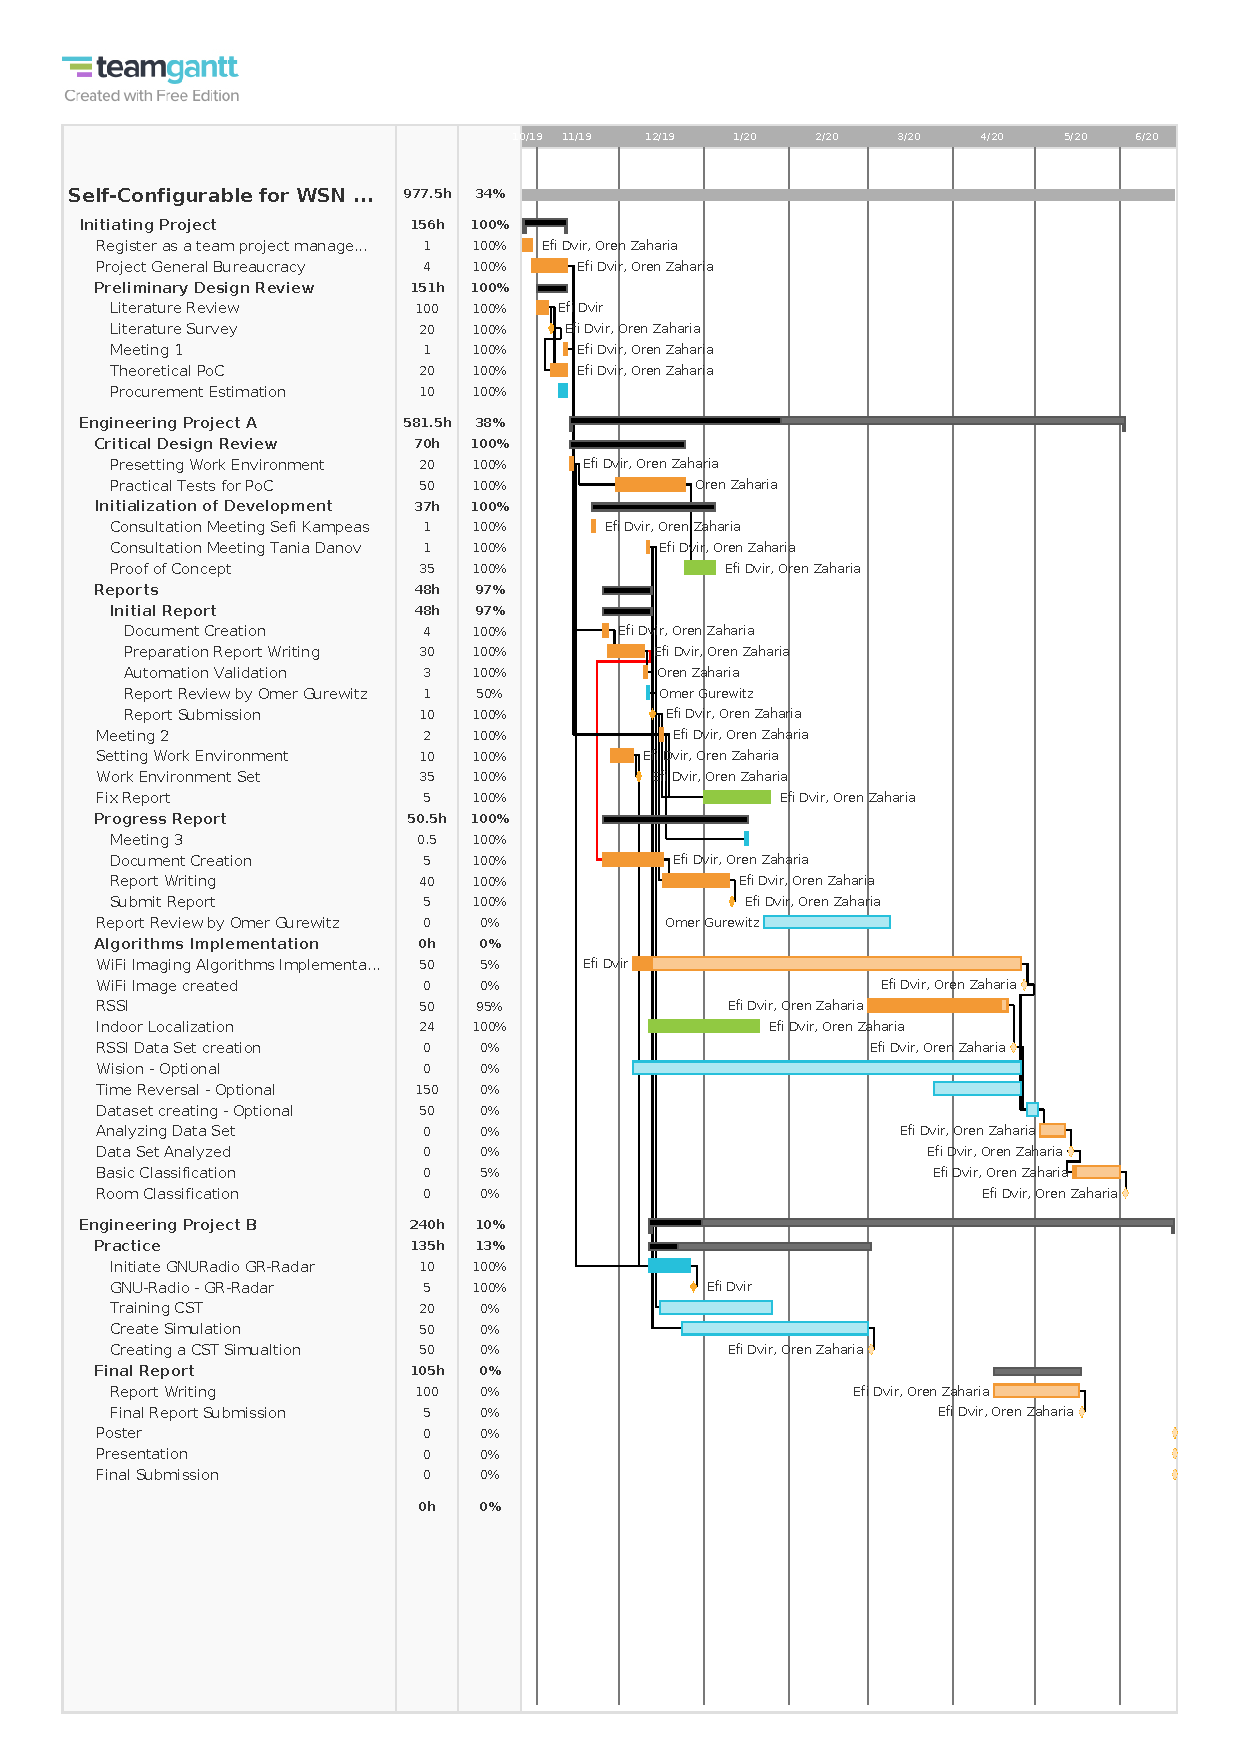
\includepdf[scale=0.68,pages=1,pagecommand=\section{Gantt}]{Self-Configurable_for_WSN_using_Wireless-Sensing.pdf}
%%%\chapter{Individual Contributions}%%%

%%%\chapter{Acknowledgements}%%%

%%%\chapter{Appendix}%%%

%%%\chapter*{Nomenclature}%%%

%%%\addcontentsline{toc}{chapter}{Nomenclature}%%%
\chapter{Progress}
\section{Achieved Objectives}
\subsection{\gls{rssi} Distance Measurements}
We've used two different formulas to estimate the distance of the \gls{wifi} client from its neighbors \acrshort{ap}. The first formula is given by the \acrshort{itu} \cite{wiki:itu_model}
\begin{equation}
    L=20\log_{10}f+N\log_{10}d+P_{f}\left(n\right)-28    
\end{equation}
where,\newline
$L$ the total path loss in dB.\newline
$f$ is the frequency in usage.\newline
$d$ the distance in meters.\newline
$n$ the number of floors between the two nodes.\newline
$P_{f}$ the floor loss penetration factor.\newline
$28$ a constant that is given in the model.\newline
\newline
Our interpretation to this model is given by 
\begin{equation}
    d=\exp\left(\log10\cdot\frac{L-20\log_{10}f-P_{f}\left(n\right)+28}{N}\right)
\end{equation}
where the results of the distance $d$ are shown in figure \ref{fig:esp_rssi}.
Another model by A.Goldsmith \cite[p.46]{goldsmith_2005}, simplified path-loss given by,
\begin{equation}
    P_{r}=P_{t}+K-10\gamma\log_{10}\left[\frac{d}{d_{0}}\right]
\end{equation}
where,\newline
$P_{r}$ is the received power (\gls{rssi}).\newline
$P_{t}$ is the transmitted power.\newline
$K$ is a unit-less constant that depends on the antenna characteristics.\newline
$\gamma$ is the path-loss exponent.\newline
$d_{0}$ is the refrenced distance [10-100]m.\newline

Our interpretation to this model is given by 
\begin{equation}
    d=\exp\left(\log10\cdot\frac{P_{t}-P_{r}+K}{10\gamma}\right)\cdot d_{0}
    \label{distance_simplified_equation}
\end{equation}

This implementation was done using the device branded by WeMos D1 and is given in figure \ref{fig:wemosd1}.
\begin{figure}[H]
\centering
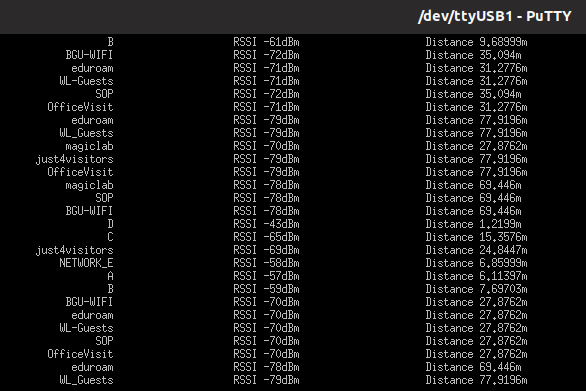
\includegraphics[width=12cm,keepaspectratio]{figures/esp_rssi.png}
\caption{Results of \gls{rssi} based distances}
\label{fig:esp_rssi}
\end{figure}
In figure \ref{fig:esp_rssi} appears a list of all the surrounding \acrshort{ssid}s broadcasted from nearby \gls{ap}s in range.
The list includes the \acrshort{ssid}, the \gls{rssi} and the calculated distance (using formula \
\ref{distance_simplified_equation}) respectively. 
The WeMos D1 node is running an operation system known as \href{https://micropython.org}{MicroPython}, and the python code that runs it, is at appendix \ref{apdx:wemos_python}.
\begin{figure}[H]
\centering
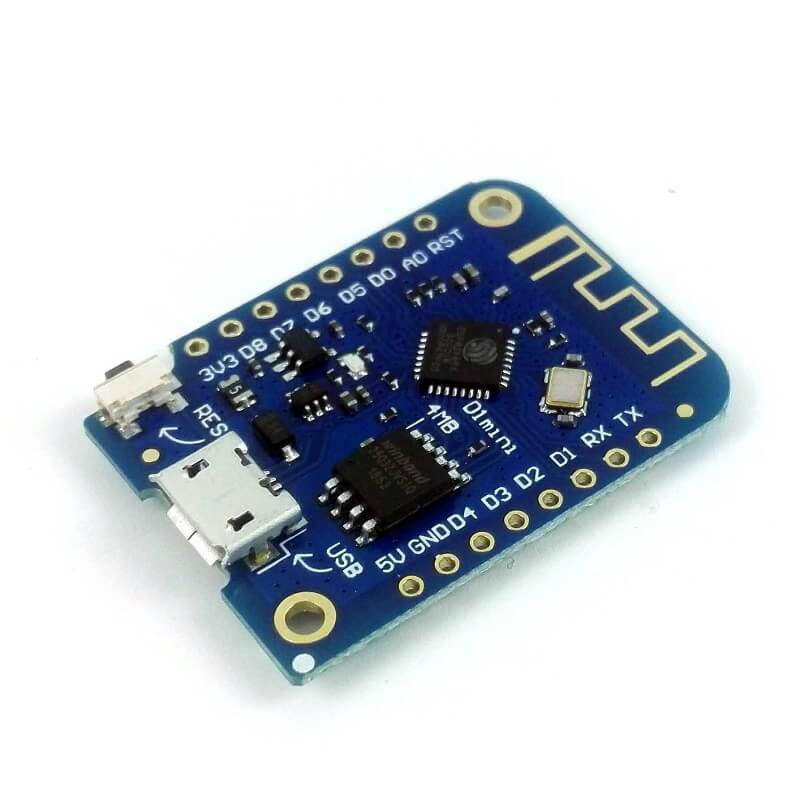
\includegraphics[width=8cm,height=6cm,keepaspectratio]{figures/wemos_d1.jpg}
\caption{\href{https://wiki.wemos.cc/products:d1:d1_mini}{WeMos D1 mini}}
\label{fig:wemosd1}
\end{figure}

\subsection{\gls{rssi} Indoor Localization}
This method described in \cite{Fundamentals_of_Wireless_Sensor_Networks} and is based on the previous paragraph, where the localization is calculated by the following equation
\begin{equation}
    \mathbf{A}\mathbf{x}=b
\end{equation}
where,\newline
$\mathbf{x}$ is the vector unknown sensor location  $\left(x,y\right)$ compared to the other anchors.
$\mathbf{A}$ is the matrix of the $n-1$ anchors compared to the sensor location, given by
\begin{equation}
    A=\left[\begin{array}{cc}
2\left(x_{n}-x_{1}\right) & 2\left(y_{n}-y_{1}\right)\\
2\left(x_{n}-x_{2}\right) & 2\left(y_{n}-y_{2}\right)\\
\vdots & \vdots\\
2\left(x_{n}-x_{n-1}\right) & 2\left(y_{n}-y_{n-1}\right)
\end{array}\right]
\end{equation}
$b$ is the vector of distances and locations of the other anchors and to the other anchors, given by
\begin{equation}
    b=\left[\begin{array}{c}
r_{1}^{2}-r_{n}^{2}-x_{1}^{2}-y_{1}^{2}+x_{n}^{2}+y_{n}^{2}\\
r_{2}^{2}-r_{n}^{2}-x_{2}^{2}-y_{2}^{2}+x_{n}^{2}+y_{n}^{2}\\
\vdots\\
r_{n-1}^{2}-r_{n}^{2}-x_{n-1}^{2}-y_{n-1}^{2}+x_{n}^{2}+y_{n}^{2}
\end{array}\right]
\end{equation}

\begin{figure}[H]
    \centering
    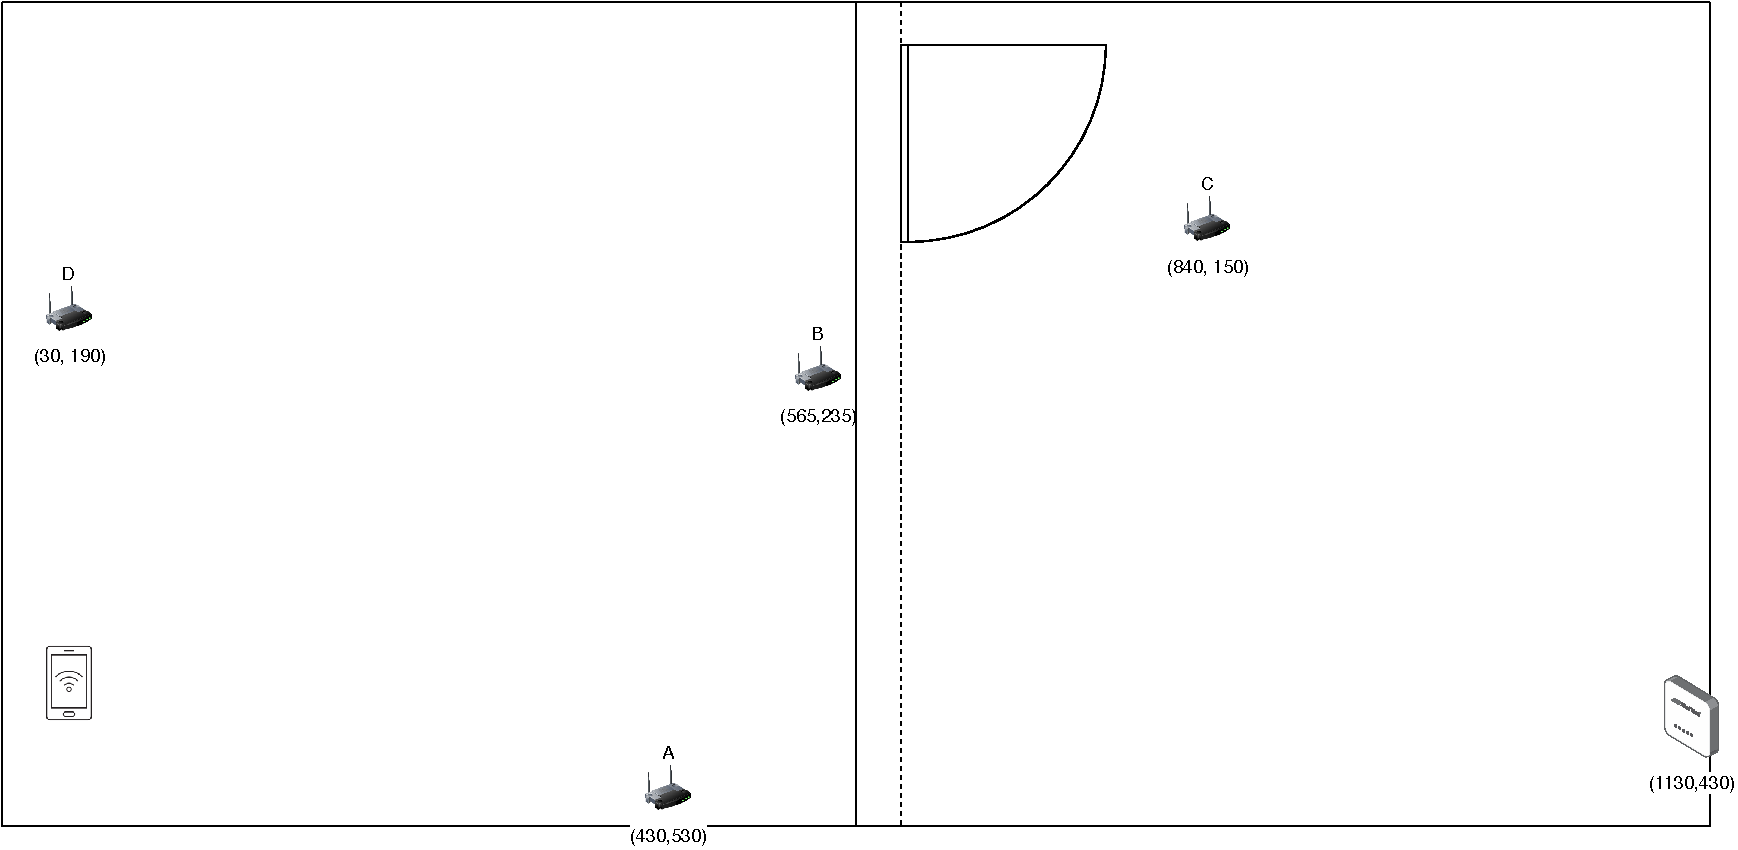
\includegraphics[height=5cm,height=5cm,keepaspectratio]{figures/Room512.pdf}
    \caption{\gls{rssi} triangulation inside 512/37 lab}
    \label{fig:rssi_triag_512}
\end{figure}
Given the figure \ref{fig:rssi_triag_512} of our space, the indoor localization, is calculated using the interpreted equation
\begin{equation}
    \left(x,y\right)=\left(\mathbf{A}^{T}\mathbf{A}\right)^{-1}\mathbf{A}^{T}b
\end{equation}
where, the distances $r_{i}$ are calculated using one of the model mentioned before, and the inverse of the matrices is calculates using the Moore-Penrose inverse methods that is pseudoinverse \cite{wiki:moorepenrose}.
The jupyter notebook code is in the appendix \ref{apdx:jupyter_indoor}.
\newline
\newline
We placed 4 \gls{wifi} routers in lab 512 and 521 and measured their location using a measuring meter.  Each router broadcasts a \gls{ssid} (A, B, C, D) which serve as an anchor  point in space. The algorithm is dependent of these points to calculate the estimated location of a sensor relative to these points.
\chapter{Bibliography}
%%%\addcontentsline{toc}{chapter}{Bibliography}
\printbibliography[type=book,heading=subbibliography,title={Books}]
\printbibliography[type=article,heading=subbibliography,title={Articles}]
\chapter*{References}
\addcontentsline{toc}{chapter}{References}
\printbibliography[type=misc,heading=subbibliography,title={Miscellaneous}]

\begin{appendices}
\chapter{Codes}
\addtocontents{toc}{\protect\setcounter{tocdepth}{0}}

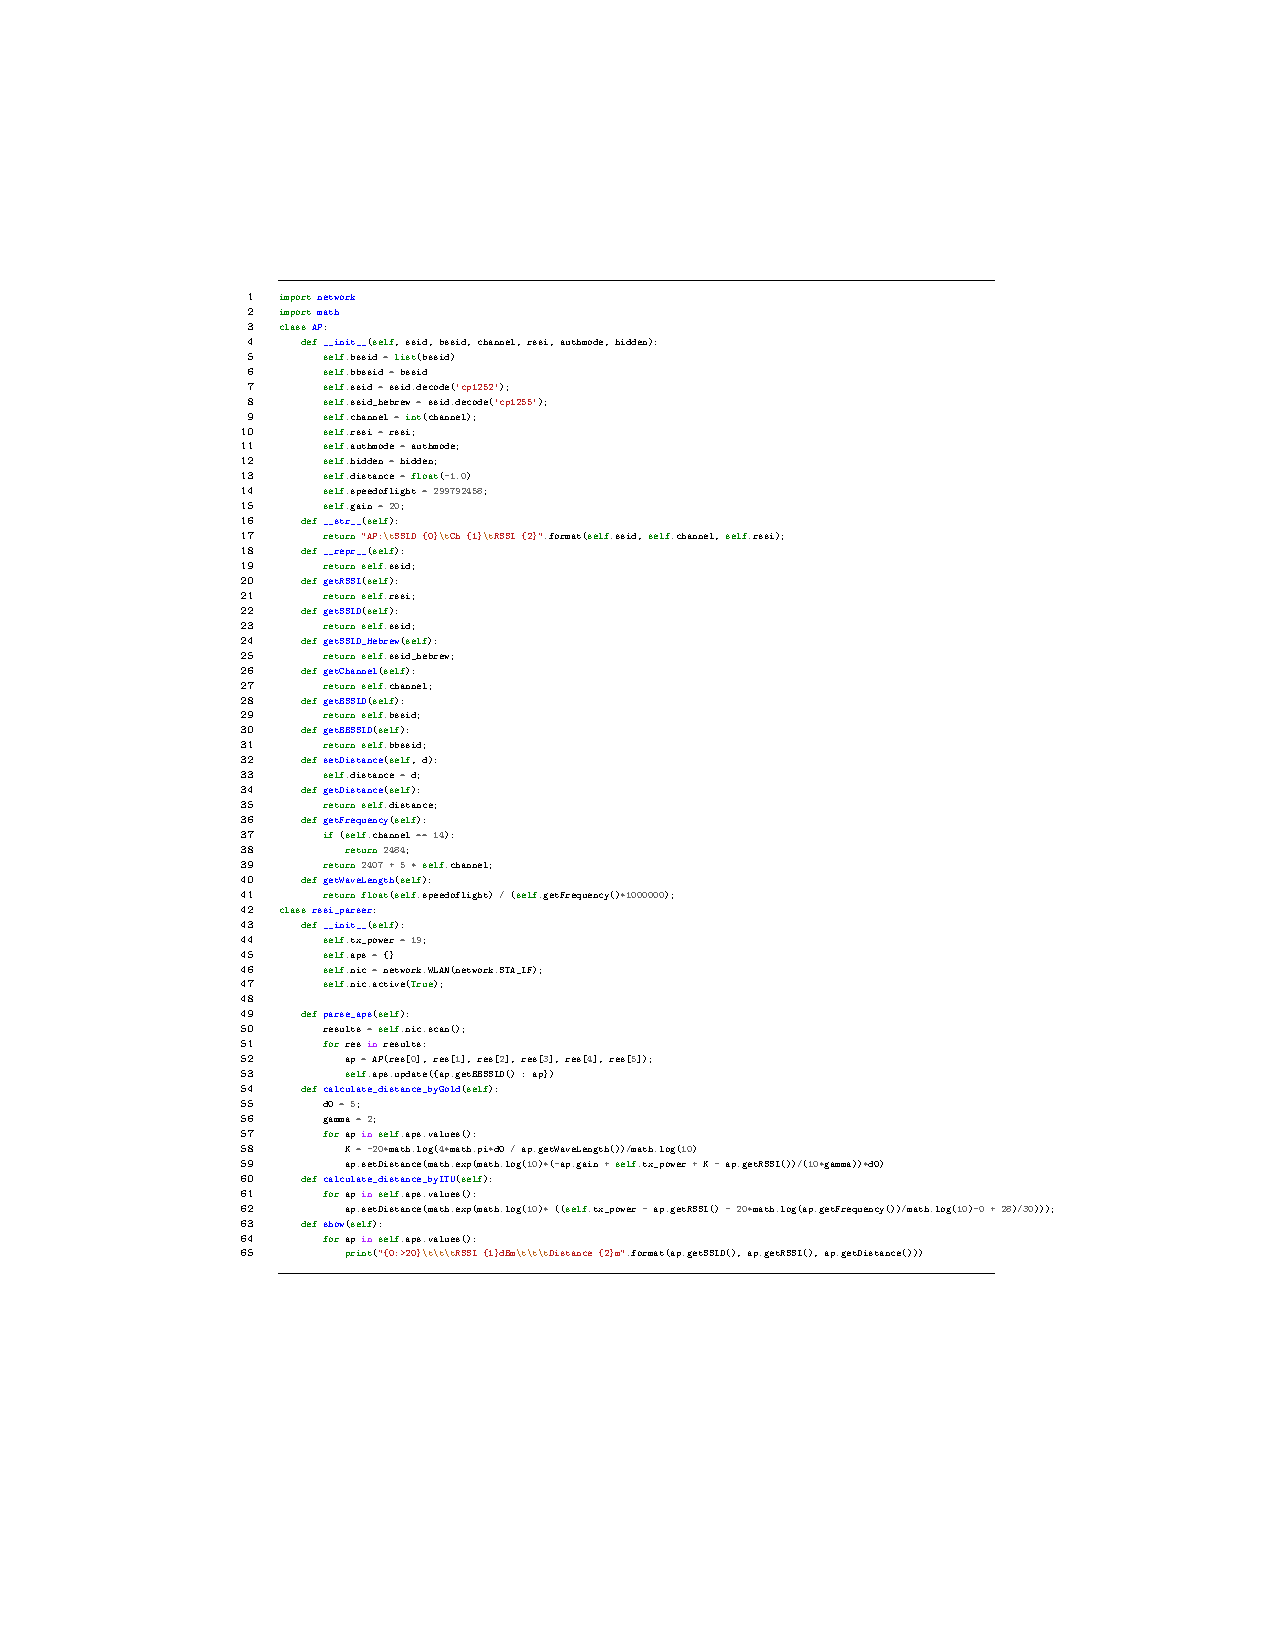
\includepdf[scale=0.9,pages=-,pagecommand={\section{MicroPython code }\label{apdx:wemos_python}}]{Python_Code.pdf}
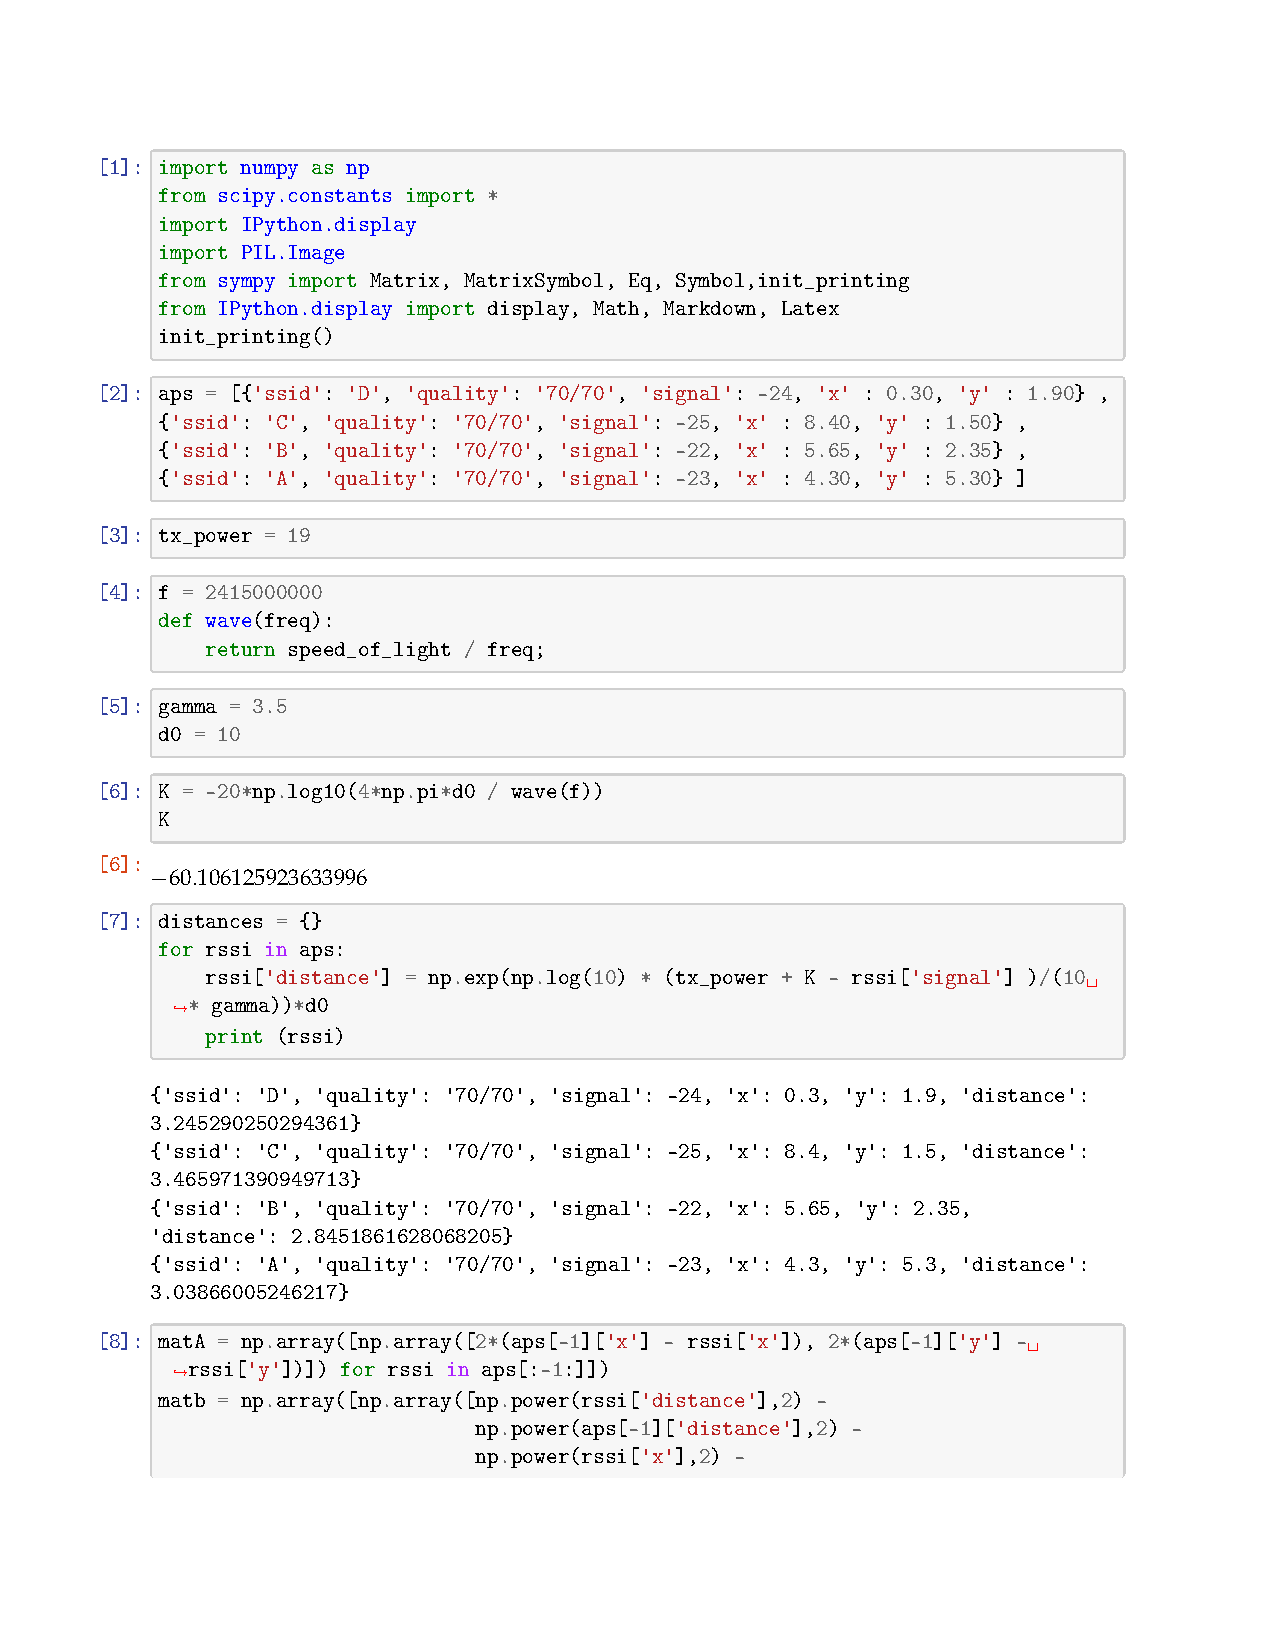
\includepdf[scale=0.75,pages={1-2},pagecommand={\section{Indoor Localization Notebook}\label{apdx:jupyter_indoor}}]{jupyter_indoor_loc.pdf}

\end{appendices}


\end{document}

